\documentclass[buriama8_dp.tex]{subfiles}
\begin{document}

\chapter{Robotic hardware and framework}

\section{ROS}
\label{sec:ros}

The arm (and the whole TRADR robot) run under the \emph{Robot Operating System} – ROS \cite{ros_paper}. This framework allows us to build robot software in a very modular fashion by providing us with standardized units (\uvz{nodes}) and M-to-N communication links (\uvz{topics}). Each hadrware component of the robot (e.g. a LIDAR or a motor driver) has its own driver node, and so does each functional software part (mapping, adaptive traversability etc.). In ROS, we can put these ready-made parts together easily, as well as design small and manageable pieces of software that integrate well with the rest of the environment and provide the new functionality we want.

The ROS framework is only a common interface specification, with the actual implementation of a node completely imdependent on other nodes. Each node can be implemented in a different programming language, as long as they conform with the communication standards.

\subsection{ROS primitives}
\label{subsec:ros_prims}

Basic unit of information in ROS are \emph{messages}. A message is a tuple with named values of different types, possibly other messages. A Pose message, representing position and orientation of an object in space, contains a Position message (which in turn contains \m x, \m y, and \m z coordinates as floating point numbers) holding the information about the position of the object, and a Quaternion representing its orientation.

The basic comminucation links are \emph{topics}. Nodes write messages to topics, and other nodes can subscribe to the topics and consume messages from them. For example a sensor driver node publishes the sensor measurements for the rest of the system to use.

The second communication primitive provided by ROS core are \emph{services}. Services implement reques-response bahavior, when a client calls the service provided by a node and receives a response for its request. For example, a laser range meter driver could be implemented as a service, accepting requests for measurement and returning the outcome.

\subsection{Actions}
\label{subsec:ros_actions}

On top of these primitives, another interface type is implemented, the \emph{actions}. Actions are not a part of core ROS, but have become \emph{de facto} a standard part of ROS interfaces. \TODO{Cite?}

 Actions consist of a set of topics and and are similar to services. A client sends a request to the action server. The action server then sends feedback back to the client as it performs the requested action. When the server is done, the client is notified by a goal message.

A good example for an action server is one for driving hte robot to a defined pose. The action server receives a Pose message and sets off. As the robot is under way, the server sends periodic updates on the current pose back to the client. When the final pose is reached, the server notifies the client that the work is done together with optional complimentary data, like the length of the path taken.


\section{Kinova JACO}
We will be working with the Kinova JACO robotic arm. It is a 6 degrees of freedom lightweight robotic arm, designed by Kinova Robotics for use in assistive and collaborative applications. As it is meant to be mounted on mobile structures as wheelchairs, JACO's lightness makes it ideal for uses on mobile robots.

\subsection{Arm kinematics}
\label{subsec:arm_kinematics}

The arm has slightly unusual geometry in its wrist. The wrist is not spherical (the axes of its joints do not intersect in one point), but consists of three revolute joints that have angular offsets of \(60\degr\) (see Figure~XX). This limits the workspace where the arm has full 6DOF capabilities, as the rotation of the wrist is limited. Usage of some inverse kinematics solvers is also impossible due to the non-standard geometry.

\subsection{Arm workspace}
\TODO{}

\subsection{Kinova ROS driver}
\label{subsec:kinova_ros}

The manufacturer provides an opensource ROS library to operate the arm \cite{kinova_ros}. The driver runs a \REV{single node} that communicates with the arm via a USB interface and relays incoming commands from other components.

The driver provides interfaces to moving the arm to joint space and carthesian space targets, controlling fingers of the gripper and directly driving carthesian velocity of the end effector and angular velocities of each joint \cite{kinova_ros_api}. It also provides two utility services for homing the arm and for stopping all movement immediately.

\subsection{Carthesian and joint space targets}
\label{subsec:api_cart_action}

Driving the arm to joint space and carthesian space targets is possible via the respective action servers. The action servers accept Pose, resp. JointAngles message describing the desired target state. They report the current position back as the movement proceeds, and in the end return the actual pose the arm ended in. For the carthesian pose target, no IK computation is performed by the driver itself, the target pose is only fed into the arm and the internal control algorithms take care of the rest. The movement also does not take any obstacle avoidance or collision prevention into accout. \REV{Self collisions are checked though.}

\subsection{Carthesian and joint space velocity}
\label{subsec:api_cart_vel}

Controlling the arm movement via diretly specifying velocities is implemented quite differently. To set carthesian or joint angular velocities, the client publishes a message to a specified topic. The driver then forwards the message to the arm, where it is consumed from a queue by the arm's control algorithm. The control algorithm runs at 100\,Hz, and sets the velocity for the next iteration from the queue. Thus, once the client stops publishing to the topic, the movement stops immediately. The control is arguably implementd this way to minimize latency of stopping any movement. It also means, that to set the velocity for a longer time, the client needs to publish to the velocity control topic periodically at 100\,Hz. With lower frequency, the movement will be jagged, as some control loop iterations will set zero velocity. If the frequency were higher, the input queue of the arm would overflow, causing the arm to stall.

\subsection{Utility services}
\label{subsec:api_util}

Homing the arm is possible by calling a home service in the ROS driver. The home pose can be adjusted in the arm firmware by Kinova's arm controlling software.

The stop service stops all movements of the arm immediately. To resume operation, the arm must be started again by calling a start service. When restarted, all commands that came after stopping are dropped and need to be re-issued if they are to be carried out.


\section{MoveIt!}
\label{sec:moveit}

The ROS framework was primarily designed to operate whole mobile robots; it is not so well suited to control robotic manipulators. To help in this area, the MoveIt! package was designed to facilitate this task. It encompasses the full stack neccessary to operate a robotic arm, from managing the state of the scene, through manipulation, motion planning, collision-checking, IK solving to outputting commands that can be used directly to control a manipulator.

\subsection{MoveIt! architecture}
\label{subsec:mvt_arch}

MoveIt runs a large monolithic node called move group. The move group is responsible for all the operations of the arm. It consumes the state of the arm (joint angles) from the driver, as well as commands from the user issued via client libraries. The architecture is illustrated in Figure~\ref{fig:moveit_arch}.

\begin{figure}[ht]
  \centering
  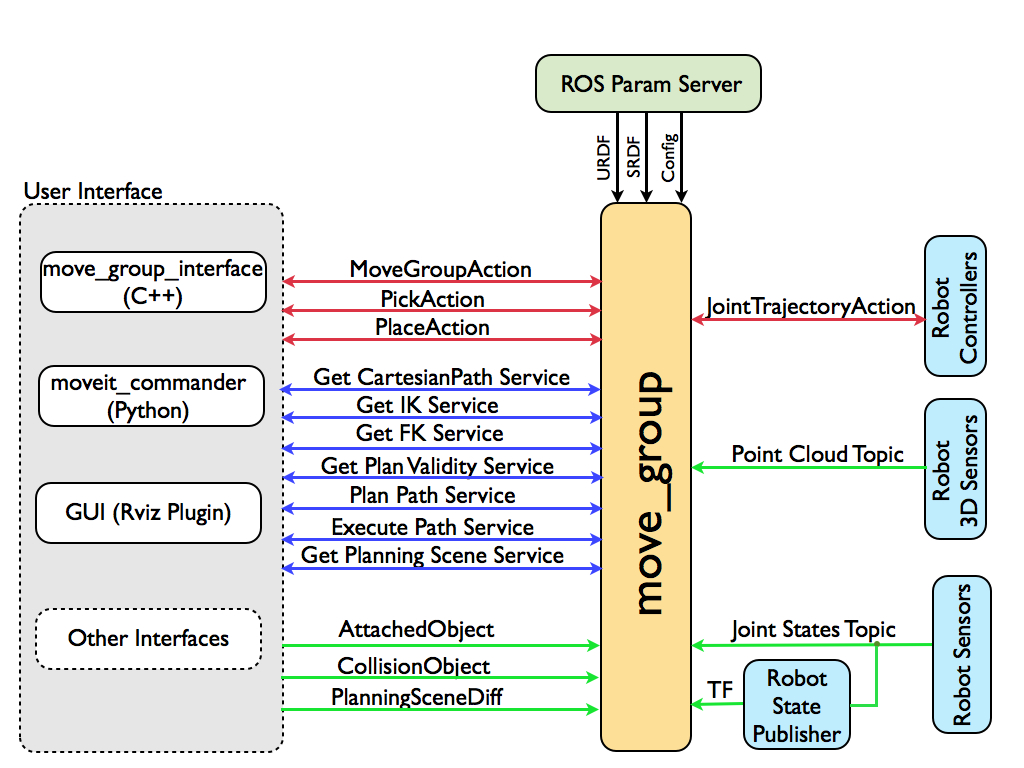
\includegraphics[width=.9\textwidth]{moveit_arch}
  \caption[MoveIt! architecture]{Illustration of MoveIt! atchitecture. Taken from \cite{moveit_docs}}
  \label{fig:moveit_arch}
\end{figure}

The central node represents the move\_group, which listens to input from the robot hardware in the lower right, as point cloud sensors and introceptive sensors. It outputs commands to the manipulator to the controller with JointTrajectoryAction interface and is controlled by the inputs on the left. 

\subsection{User interface}
\label{subsec:moveit_ui}

The user interface, or client libraries, for MoveIt are prepared in C++ and python. The libraries contain objects and utility functions to use the functionality of the move group and communicate with the move group via its ROS topic and service interface. All the interfaces and functionalities are very poorly documented, and the best available resources are the automatically generated code documentation and the source code itself. The client libraries can be used directly to access the motion planning capabilities to reach some higher-level goals.


\subsection{Robot interface}
\label{subsec:moveit_ri}

MoveIt interfaces with the robot hardware by an action server implementing the JointTrajectoryAction. The server then drives the arm hardware. The JointTrajectoryAction is specified as a trajectory in space of joint velocities, prepared by the motion planner with respect to both the arm kinematics (preventing collisions) and the arm dynamics (taking limits on joint acceleration into account).

In case of the Kinova ROS driver, no such server is provided by the manufacturer. A pull request on Github containing this functionality exists, but is not a part of the release yet. We used an implementation of this server by \REV{Matěj Balga}, which we updated to work with the newest drivers from Kinova.

\subsection{Arm simulator}
\label{subsec:arm_sim}

\TODO{Describe fake arm driver}

\subsection{Inverse Kinematics solver -- TRAC-IK}
\label{subsec:tracik}

During our initial experiments with the arm, we encountered puzzling behaviors of the motion planners. The arm would sometimes move along a seemingly random, unneccessarily long path. At closer investigation, we concluded that the planning was actually optimal, but what was wrong was the Inverse Kinematic (\emph{IK}) solution for the target pose.\TODO{Illustrate!}

\TODO{Present IK?}

Because of the slightly non-standard arm kinematics (see section \ref{subsec:arm_kinematics}), the default IK solver used by MoveIt (the KDL numerical solver) would sometimes produce a solution that indeed reaches the desired end effector pose, but that is very far in joint space from the current joint state, even when a very small end effector motion is required.

\begin{figure}[ht]
  \centering
  \TODO{Different configurations image and description}
  %\includegraphics[options]{figures/path.pdf}
  \label{fig:label}
  \caption{}
\end{figure}

This is caused by the KDL implementation. KDL finds the IK solution by iterating iteratively.

\TODO{Should the algorithm be here? Exclude it completely?}
\begin{algorithm}[htp]
\begin{algorithmic}
  \State \textbf{Input:} \(\vec p \gets\) desired target carthesian pose
  \vspace{1em}

  \State \(\vec q \gets\) seed joint values
 
  \Do
    \State \(\vec p_c \gets\) computeFK(\(\vec q\))
    \State \(\mat J \gets\) computeJacobian(\(\vec q\))
    \State \(\vec e \gets \vec p_c - \vec p\)

    \State \(\vec q \gets \vec q + \mat J^+ \vec e \)
  \doWhile{\(|e|<\epsilon\)}

  \vspace{1em}
  \State \textbf{return} \(\vec q\)
\end{algorithmic}
\caption{KDL iterative IK solver}
\label{alg:kdlik}
\end{algorithm}

This approach is analogic to using the Newton method to minimize the carthesian space error. The Jacobian matrix \(\mat J\) is a matrix of partial derivatives where
\[
\mat J_{i,j} = \frac{\pdiff{\vec p_i}}{\pdiff q_j}
\]
\marginpar{\TODO{revise \(i,j\)}}
and thus
\[
\mat J_{i,j}^{-1} = \frac{\pdiff{\vec q_j}}{\pdiff p_i}.
\]
and by iteration in Algorithm~\ref{alg:kdlik} we descend the pose error by preforming its local linear approximation and taking a step that minimizes it. The pseudoinverse is used in KDL because \quot{it is more efficient to compute}{tracik}, \REV{ while it is numerically more stable}.

The descent can get trapped in local minima when some of the joints limits are reached. This is solved by restarting the search from a random seed position. Then, the found position can be one very distant from the original position in joint space.

This issue is tackled by a new IK solver released recently, TRAC-IK \cite{tracik}. The solver implements another approach to solving the IK problem by formulating it as a Sequential Quadratic Programming problem, minimizing \(|e|^2\) with joint limits as constraints. The solver also allows the user to spedify other constrints, like a wish to minimize joint-space distance between the seed (current arm joint values) and the result.

This setting allows us to eliminate the large joint space changes for minor movements, which was an issue with the JACO arm before.

\section{Tactile sensing}

Previous work in the field of tactile exploration at FEE \cite{vojta} used effort readings from the arm joints to detect tool contact when exploring terrain. To prevent arm damage, the movement had to be very slow, making it painstaking to explore event very little of the environment.

To improve exploration efficiency, we used a 3D force sensor to detect whether our tool is in contact with the environment. This allows us to move the arm much faster with confidence that we will be able to stop the arm with latency low enough to guarantee the arm nor the force sensor would be harmed.

\subsection{Optoforce sensor}
\label{subsec:opto}

The force sensor used is an Optoforce OMD-20-SE-40N sensor. Optoforce sensors represent a novel approach to 3D force sensor construction, as their working principle enables them to be made very rugged, resilient.


\begin{figure}[ht]
  \begin{subfigure}[t]{0.4\textwidth}
    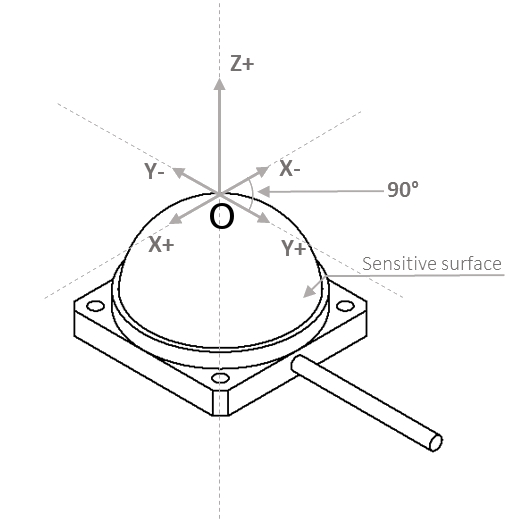
\includegraphics[width=\textwidth]{OMD-sketch-with-axises}
    \caption{}
    \label{fig:omd_geom}
  \end{subfigure}
  \begin{subfigure}[t]{0.4\textwidth}
    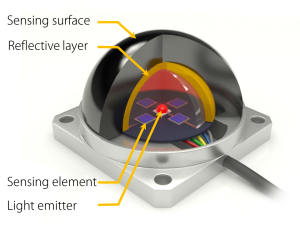
\includegraphics[width=\textwidth]{OMD-xsec}
    \caption{}
    \label{fig:omd_xsec}
  \end{subfigure}

  \caption[Optoforce sensor]{\TODO{Cite}}
  \label{fig:decomps}
\end{figure}


The Optoforce sensor, seen in cross-section in Figure~\ref{fig:omd_xsec}, consists of an aliminium base plate, made in different designs, and a hollow silicone hemispherical dome. The interior of the dome is coated with a reflective layer. A light emitter, IR LED, is positioned on the base plate in the center of the dome. Four light-sensitive diodes are placed around it.

When the sensor is operational, the LED emits light which bounces around the dome and provides known, constant illumination on the photodiodes. When force is applied to the dome, it deforms, and the deformation causes the illumination of the diodes to shift. From this shift, it is possible to determine the direction in which the force has been applied. According to the manufacturer, deformations in range of hundreds of nanometers can be measured \cite{opto_whitep}.

The sensor has its own DAQ module, which communicates with a computer via a serial link emulated over USB. The manufacturer provides a C++ library that exposes the sensor functionality in an API. It however depends on the problematic Qt framework. Shadow Robot Company \cite{opto_driver}  implemeted a ROS node that connects to the sensor serial interface, configures sensor parameters like measurement and filter frequency, reads the data output by the sensor and publishes them on a ROS topic to be proessed by other components. The software was released under GPLv2. We simplified the driver and slightly adjusted it to work better in our setup.

\subsection{Sensing tool}
\label{subsec:sense_tool}

The Optoforce sensor is relatively small. Mounting it on the JACO arm and using it to sense direct contact with an obstacle would mean the arm would get uncomfortably close to it. We devised a way to extend the sensor so that force readings are taken not at the sensor dome, but at a stick. This increases the arm range and makes it possible to keep the arm safely away from unknown obstacles.


\begin{figure}[ht]
  \centering

  \begin{subfigure}[t]{0.49\textwidth}
   \label{fig:opto_frame}
   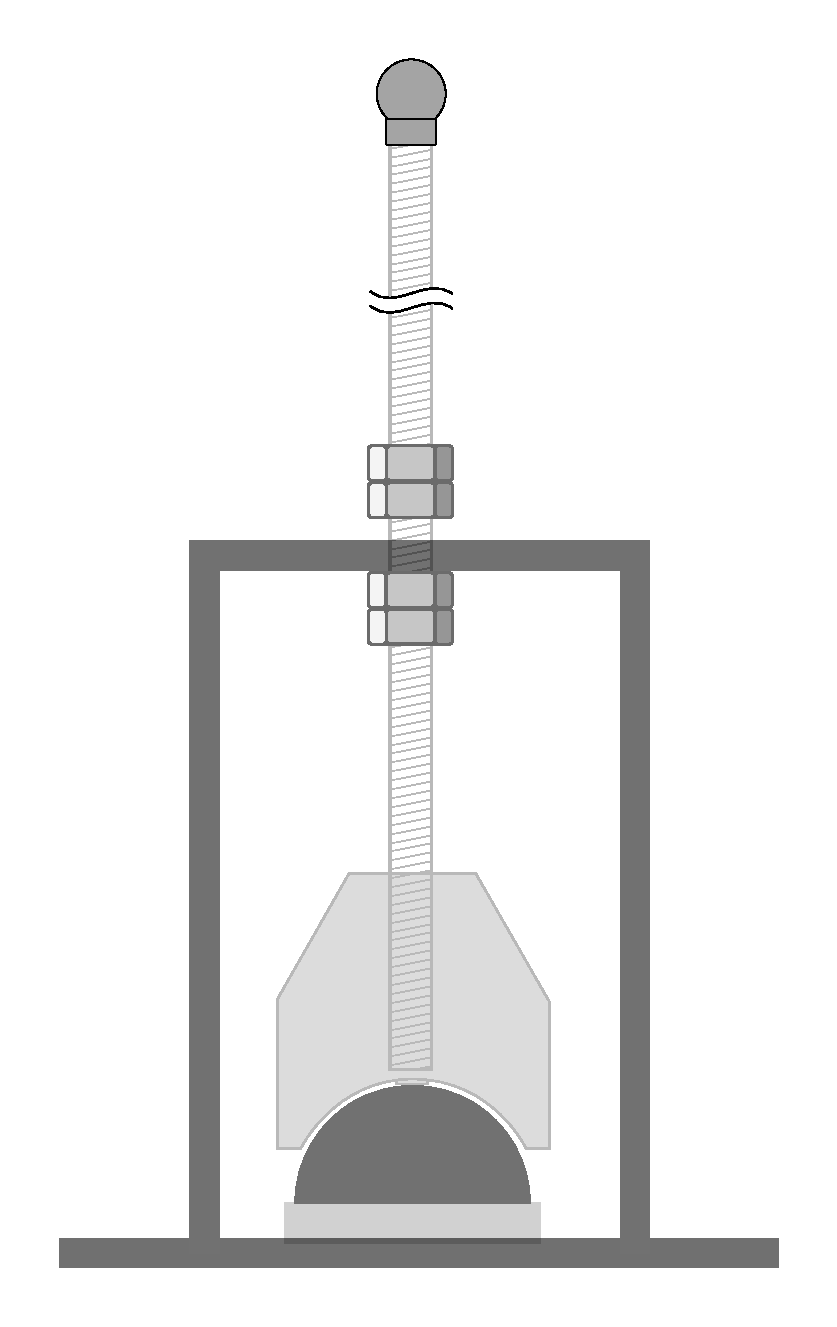
\includegraphics[width=\textwidth]{otpo_frame.pdf}
   \caption{}
  \end{subfigure}
  %
  \begin{subfigure}[t]{0.49\textwidth}
   \label{fig:frame_forces}
   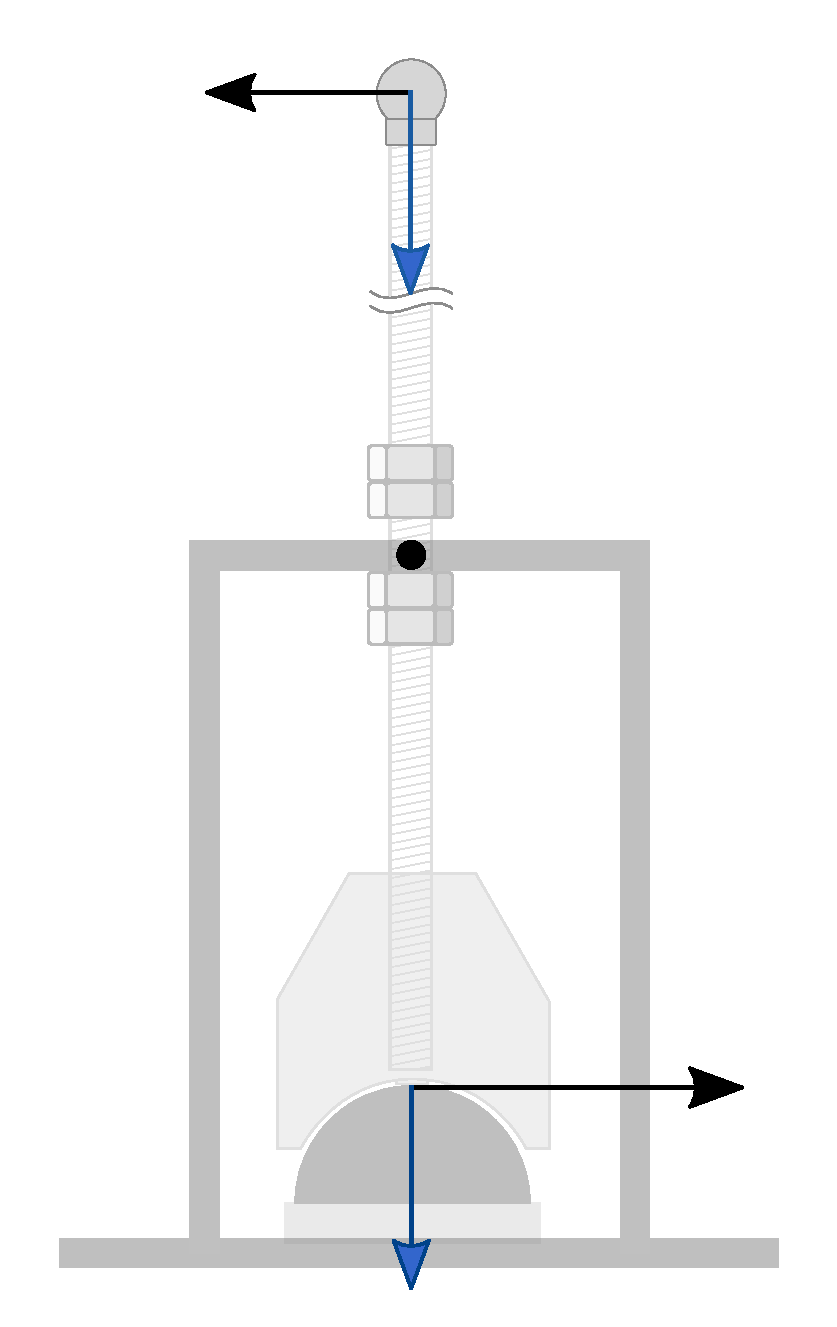
\includegraphics[width=\textwidth]{otpo_frame_forces.pdf}
   \caption{}
  \end{subfigure}

 \caption[Sensing tool]{The sensing tool assembly.}
 \label{fig:opto_frame}
\end{figure}


\begin{figure}[ht]
  \centering
  \TODO{Photo of whole setup}
  %\includegraphics[options]{figures/path.pdf}
  \caption{}
  \label{fig:label} 
\end{figure}

The stick acts as a lever with the pivot point being the assembly frame. When a lateral force is applied to the stick, the sensor records force in oppposite direction. Axial force is applied directly to the sensor. The principle is illustrated in Figure~\ref{fig:frame_forces}.

The sensor dome is in contact with a cap attached to the stick. The cap is pressed against the dome with a preloaded force, to ensure accurate measurement of even very small forces applied to the stick. The deformation of the dome is limited by a pair of nuts that limit the travel of the stick.




\subsection{Measurement processing}
\label{subsec:opto_process}



\end{document}

%%% Local Variables:
%%% mode: latex
%%% TeX-master: "buriama8_dp"
%%% End:
